\chapter{Implementation}
\label{ch:Implementation}

This chapter describes the theoretical design of the filter algorithm proposed in \cite{bennett_motion_2014} as well as its implementation, based on the fundamentals acquired in the previous chapters. Other than \citeauthor{bennett_motion_2014} in \cite{bennett_motion_2014} who tested the filter algorithm by hand, we used movement data from real subjects. After outlining the initial situation, i.\,e. stating existing orientation algorithms, the theoretical design of the filter is described in detail. Subsequently, the software implementation and experiments are given, followed by the results and their discussion.

\section{Initial Situation}

There was already a variety of algorithms implemented, in order to estimate the pitch angle of the thighs and shanks based on data gathered with the GaitWatch system. The existing ones are described below.

\begin{itemize}
  \item \textsc{projection of the gravity vector:} One way to obtain the pitch angle from the inertial data is using the projection of the gravity vector on the axes of the accelerometer, as described in Section \ref{sec:projection_gravity}. The first algorithm computed the pitch angle according to Equation \ref{eq:projection_gravity}.
  
  \item \textsc{integration of the angular rate:} Another way to obtain the pitch angle is the integration of the angular rate, as outlined in Section \ref{sec:integration_angular}. There are many different numerical integration methods that can be used. The existing algorithms used the approximation of the integral according to the trapezoidal rule
  
  \begin{equation}
   \theta(n) = \theta_0 + \int_{0}^{n T_s} \omega(t)\, dt \approx \theta_0 + \frac{T_s}{2} \sum_{k=1}^{n} \left[ \omega_{k} + \omega_{k-1} \right]\,,
  \end{equation}
  
  \noindent
  where $n, k \in \mathbb{N}$ denote time normalised to the sample period $T_s$, $\omega_k$ the measured angular rate at instant $k$, and $\theta_0$ the angle at $k=0$. The implemented algorithm computed the angle recursively as
  
   \begin{equation}
   \theta(n) \approx \theta(n-1) + \frac{T_s}{2} \left[ \omega_{k} + \omega_{k-1} \right]\,, \quad \theta(0) = \theta_{0}\,.
  \end{equation}
  
  \item \textsc{kalman filter:} The third algorithm fused the orientation angle based on the projection of the gravity vector with the gyroscope measurements from a single sensor in a classic kalman filter, without taking the motion intensity into account \cite{olivares_vicente_gaitwatch_2013}.
  
  \item \textsc{gated kalman filter:} This algorithm extended the aforementioned one by setting the measurement noise covariance according to the motion intensity \cite{olivares_vicente_gaitwatch_2013} and was already mentioned in detail in Section \ref{sec:state_of_the_art_kalman}.
  \end{itemize}

In tandem with an orientation estimation based on a Qualisys motion capture system using cameras in combination with optical markers, these orientation algorithms served as a reference. The placement of the markers on the leg are depicted in Figure \ref{fig:marker_placement}. From the recorded motion of the markers in space the motion capture system computed the orientation angles of the thighs and shanks.

\begin{figure}
\centering
	\begin{tikzpicture}[auto, thick, node distance=3cm,>=latex']
    \pgftext{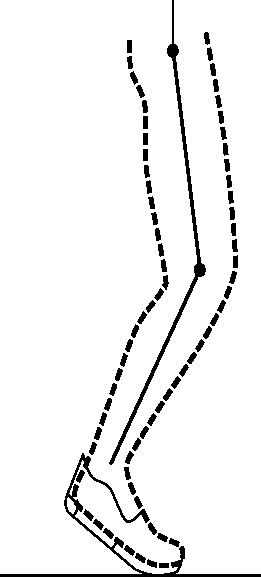
\includegraphics[width=3.5cm]{images/sensors_on_leg}} at (0pt,0pt);
    \node [] (a) at (-4.4, -2) {};
    \node [] (b) at (-4.5, 0.1) {};
    \node [] (c) at (4.45, 3.3) {};
\end{tikzpicture}
\caption{Human leg with optical markers, from \cite{tao_gait_2012}.} \label{fig:marker_placement}
\end{figure} 

\section{Theoretical Design}\label{sec:theoretical_design}

This section maps the theoretical design of the system proposed by \citeauthor{bennett_motion_2014} in \cite{bennett_motion_2014} to the existing GaitWatch system. It states the assigned coordinate frames and the conventions with respect to rotations about their axes. Furthermore, it describes the kinematic model and the extended Kalman filter in detail.

\subsection{Kinematic Model}

The \emph{kinematic model} relates the respective angles of the thigh and shank about the hip and knee joint to the acceleration seen by the wearable sensors. When walking in a straight line, the human leg can be modelled as a two-link planar revolute robot \cite{bennett_motion_2014}. Then, thighs and shanks remain in a single plane which is approximately parallel to the direction of motion. As depicted in Figure \ref{fig:robot}, the revolute joints of the pendulum robot represent the hip und knee joint, and the two links the thigh and shank, respectively. The origin of the inertial world frame is located at the base of link $1$, the upper of both links. The $x$-axis points forward, the $y$-axis points out from the hip to the right, and the $z$-axis points down. This configuration follows the right-hand rule, which can also be used to determine the sense of rotation around the axes. The pitch angle $\theta_1$ is measured with respect to the $x$-axis, and the pitch angle $\theta_2$ of link $2$ with respect to link $1$. 

\begin{figure}
\centering
\begin{tikzpicture}[auto, thick,>=latex']
	\node [draw, rectangle, minimum height=1.6cm, minimum width=1.6cm, pattern=north west lines] at (0,0) (solid) {};

    \node [draw,  fill=white, very thick, rectangle, rounded corners=3pt, minimum height=3.7cm, minimum width=1cm, align=center, rotate around={30:(0,0)}] at (0.7, -1.25) (link1) {};
    \node [draw, thick, fill=gray, rounded corners=2pt, rectangle, minimum height=0.8cm, minimum width=0.45cm, align=center, rotate around={30:(0, 0)}, label={[label distance=0.18cm]335:IMU $1$}] at (0.98, -1.7) (sensor1) {};
    
    \node [draw, fill=white, very thick, rectangle, rounded corners=3pt, minimum height=3.7cm, minimum width=0.6cm, align=center, rotate around={145:(0,0)}] at (0.6, -3.7) (link2) {};
    \node [draw, thick, fill=gray, rounded corners=2pt, rectangle, minimum height=0.8cm, minimum width=0.45cm, align=center, rotate around={145:(0, 0)}, label={right:IMU $2$}] at (0, -4.56) (sensor2) {};
    
    \node[coordinate] (X) at (2.5,0) {};
    \node[coordinate] (Y) at (0,-2.5) {};
    \node[coordinate] (O) at (-0, 0) {};
    
    \draw[->] (O) -- node[name=x] {$x$}(X);
    \draw[->] (O) -- node[pos=0.6, name=y, label={left:$z$}] {}(Y);
    
    \draw[->] (0, -4.56) -- node[name=x_2] {$x_2$}(1.5, -5.6);
    \draw[->] (0, -4.56) -- node[name=x_2] {$z_2$}(-1.1, -6.1);
   
    \draw[dotted] (O) -- (2.5,-4.3);
    \draw[fill=white] (0,0) circle (4pt);
    \draw[fill=black] (0,0) circle (1pt) node[label={[label distance=-1.2mm]180:$y$}]{};
    \draw (1.45, -2.5) circle (4pt);
    
    \draw[-stealth] (1.2,-1) arc (300:355:1.2);
    \draw[-stealth] (0.8,-4.1) arc (240:303:1.4);
    
    \node at (1.3, -0.4) (angle1) {$\theta_1$};
    \node at (1.5, -3.7) (angle1) {$\theta_2$};
\end{tikzpicture}
\caption{Kinematic model of the human leg, from \cite{bennett_motion_2014}.} \label{fig:robot}
\end{figure} 

The \glspl{IMU} placed on the thighs and shanks measured the angular velocity and linear acceleration of the thighs and shanks, respectively. According to \citeauthor{spong2005robot} \cite{spong2005robot}, the $x$ and $z$ displacement and its derivatives in the world frame are as follows:

\begin{align}
  x &= + l_1 \cos(\theta_1) + l_2 \cos(\theta_1 + \theta_2) \\
  \dot{x} &= -l_1 \dot{\theta}_1 \sin(\theta_1) - l_2 (\dot{\theta}_1 + \dot{\theta}_2) \sin(\theta_1 + \theta_2) \\
  \ddot{x} &= -l_1 [\dot{\theta}^2_1 \cos(\theta_1) + \ddot{\theta}_1 \sin(\theta_1)] - l_2 [(\dot{\theta}_1 + \dot{\theta}_2)^2 \cos(\theta_1 + \theta_2) \nonumber \\ 
  &\mathrel{\phantom{=}} + (\ddot{\theta}_1 + \ddot{\theta}_2) \sin(\theta_1 + \theta_2)] \label{eq:acc_x} \\
  \nonumber \\
  z &= -l_1 \sin(\theta_1) - l_2 \sin(\theta_1 + \theta_2) \\
  \dot{z} &= -l_1 \dot{\theta}_1 \cos(\theta_1) - l_2 (\dot{\theta}_1 + \dot{\theta}_2) \cos(\theta_1 + \theta_2) \\
  \ddot{z} {}&= -l_1 [\ddot{\theta}_1 \cos(\theta_1) - \dot{\theta}^2_1 \sin(\theta_1)] - l_2 [(\ddot{\theta}_1 + \ddot{\theta}_2) \cos(\theta_1 + \theta_2) \nonumber \\ 
  &\mathrel{\phantom{=}} - (\dot{\theta}_1 + \dot{\theta}_2)^2 \sin(\theta_1 + \theta_2)] \label{eq:acc_y}
\end{align}

\noindent
in which $l_1$ and $l_2$ are the lengths of the two links, respectively. Using Equations \ref{eq:acc_x} and \ref{eq:acc_y}, and the \emph{a priori} estimates of the angles $\theta_1$ and $\theta_2$ and their derivatives, i.\,e. the angular rates $\omega_1$ and $\omega_2$, and the angular accelerations $\alpha_1$ and $\alpha_2$, respectively, obtained with the EKF described in Section \ref{sec:EKF_model}, we can estimate the motion based acceleration in $x$ and $z$ direction that sensor $2$ will see in the world coordinate frame.

The orientation of the sensor frames at rest are different from the world frame and dynamic when the pendulum is in motion. In order to transform the values from the world frame to the dynamic body frame of \gls{IMU} $2$, which is depicted in Figure \ref{fig:robot}, we used the transformation matrix $\mathbf{T}_y(\theta)$ from Equation \ref{eq:transformation_matrices} in transposed form. The positive sense of rotation according the right-hand rule is opposite to the mathematically positive sense, which is why we use the transpose of the transformation matrix. The body frame of sensor two is not aligned with the world frame for $\theta_1 = \theta_2 = 0$. Thus, an offset of $-\frac{\pi}{2}$ is necessary. With $\theta = \theta_1 + \theta_2 - \frac{\pi}{2}$, this yields

\begin{equation}
\mathbf{T}^T_y(\theta_1 + \theta_2 - \frac{\pi}{2}) = \begin{bmatrix}
    \cos (\theta_1 + \theta_2 - \frac{\pi}{2}) \; & 0 \; & \sin (\theta_1 + \theta_2 - \frac{\pi}{2}) \\
    0 \; & 1 \; & 0 \\
    -\sin (\theta_1 + \theta_2 - \frac{\pi}{2}) \; & 0 \; & \cos (\theta_1 + \theta_2 - \frac{\pi}{2})
    \end{bmatrix}\,.
\end{equation}

\noindent
The rotated tangential and radial components of the motion based acceleration estimates, $A_{rad}$ and $A_{tan}$ are found using the tranformation matrix to rotate the results of Equations \ref{eq:acc_x} and \ref{eq:acc_y}, respectively, according to Equation \ref{eq:transformation}.

\begin{equation}
  \begin{bmatrix}
  	A_{rad} \\
  	A_{axi} \\
  	A_{tan}
  \end{bmatrix} = \mathbf{T}^T_y(\theta_1 + \theta_2 - \frac{\pi}{2}) \begin{bmatrix}
  	\ddot{x} \\
  	0 \\
	\ddot{z}
  \end{bmatrix}
\end{equation}

\noindent
The axial component is zero, since the leg is assumed to be oriented perpendicular to to the earth's surface and thus perpendicular to the $y$-axis.

Then, the radial and tangential acceleration estimates are subtracted from the sensor readings $A_x$ and $A_y$, which leaves an estimate of the gravity based acceleration $\mathbf{g}$ that acts on the sensor:

\begin{equation}
\mathbf{g} = \begin{bmatrix}
    g_x \\
    g_y \\
    g_z 
    \end{bmatrix} = 
    \begin{bmatrix}
    A_x \\
    0 \\
    A_z 
    \end{bmatrix} -
    \begin{bmatrix}
    A_{rad} \\
    0 \\
    A_{tan} 
    \end{bmatrix}\,.
\end{equation}

\noindent
According to Equation \ref{eq:projection_gravity} the angle estimate is then

\begin{equation}
  \theta_1 + \theta_2 = \mbox{atan}2(-g_z, g_x)\,.
\end{equation}

\noindent
This improved angle estimate is then fused with the estimate based on the integration of the angular rate measured with the gyroscope, in order to reduce the estimation error due to gyroscope drift.

 \label{sec:EKF_model}

The state-space model of the extended Kalman filter is given by the state vector $\mathbf{x} \in \mathbb{R}^{n=10}$

\begin{equation} \label{eq:state_vector}
  \mathbf{x} = \begin{bmatrix}
  	x, & z, & \theta_1, & \omega_1, & \alpha_1, & \theta_2, & \omega_2, & \alpha_2, & \beta_1, & \beta_2
  \end{bmatrix}^T
\end{equation}

\noindent
where $x$ and $y$ correspond to the horizontal and vertical position of the end of link $2$ with respect to the origin of the world frame, i.\,e. the hip joint. $\theta_1$ is the angle, $\omega_1$ the angular velocity, and $\alpha_1$ the angular acceleration of the first joint, respectively. The corresponding values for the second link are $\theta_2$, $\omega_2$, and $\alpha_2$. The biases from the gyroscope on the first and second sensor are $\beta_1$ and $\beta_2$, respectively. They are assumed to be constant or slowly time varying.

The measurement vector $\mathbf{z} \in \mathbb{R}^{m=3}$ is given by

\begin{equation} \label{eq:measurement_vector}
  \mathbf{z} = \begin{bmatrix} z_1 \\ z_2 \\ z_3 \end{bmatrix} = \begin{bmatrix}
  	\omega_1 + \beta_1, & \omega_1 + \omega_2 + \beta_2, & \theta_1 + \theta_2
  \end{bmatrix}^T + \mathbf{v}\,.
\end{equation}
 
\noindent
where $\mathbf{v}$ is the random measurement noise process, modelled as zero-mean, Gaussian white noise. The element $z_1$ represents the measurement of the first link angular velocity, which is the sum of the first link rotation and the gyroscope $1$ bias. The element $z_2$ represents the measurement of the second link angular velocity, which is the sum of the first and second link rotation and the bias of gyroscope $1$ and gyroscope $2$. Finally, the element $z_3$ is the angle estimate of the second accelerometer, which will see the angular displacement of both links.

According to  \citeauthor{rowell2002state} \cite{rowell2002state}, the plant dynamics of a system can be expressed as a set of $n$ coupled first-order ordinary differential equations, known as the \emph{state equations}. The modelled system is governed by the \emph{non-linear} ordinary differential equations

\begin{equation} \label{eq:state_vector_derivative}
  \dot{\mathbf{x}} = \mathbf{f}(\mathbf{x}, t) + \mathbf{w} = \left[\begin{smallmatrix}
  -l_1 \omega_1 \sin(\theta_1)  - l_2 (\omega_1 + \omega_2) \sin(\theta_1 + \theta_2) \\
  -l_1 \omega_1 \cos(\theta_1)  - l_2 (\omega_1 + \omega_2) \cos(\theta_1 + \theta_2) \\ \omega_1 \\ \alpha_1 \\ 0 \\ \omega_2 \\ \alpha_2 \\ 0 \\ 0 \\ 0
  \end{smallmatrix}\right] + \mathbf{w}\,.
\end{equation}

\noindent
where $\dot{\mathbf{x}}$ consists of the component-wise time derivatives of the state vector $\mathbf{x}$, 

\begin{equation}
  \dot{x}_i = f_i(x_1(t), \dots, x_n(t), t) + w_i = \frac{dx_i}{dt} + w_i\,, \quad i = 1, \dots, n\,,
\end{equation}

\noindent
expressed in terms of the state variables $x_1(t), \dots, x_n(t)$. Given this \emph{state-space representation}, the system state at any instant may be interpreted as a point in an $n$-dimensional state space whose axes are the state variables. The dynamic state response $\mathbf{x}(t)$ can be interpreted as a trajectory traced out in the state space. The system described by Equation \ref{eq:state_vector_derivative} is \emph{time-invariant} since it does not depend explicitly on time. Thus, we may leave out the $t$ and write from now on $\mathbf{f}(\mathbf{x}) = \mathbf{f}(\mathbf{x}, t)$.

For a \emph{linear} system in state space form given by

\begin{equation}\label{eq:linear_continuous}
  \dot{\mathbf{x}} = \mathbf{F} \mathbf{x}\,,
\end{equation}

\noindent
with a time-invariant \emph{system dynamics matrix} $\mathbf{F}$ there is a \emph{state transition matrix} $\bm{\Phi}(t-t_0)$ that propagates the state of the system forward from any time $t_0$ to a time $t$, according to

\begin{equation}
  \mathbf{x}(t) = \bm{\Phi}(t-t_0) \mathbf{x}(t_0)\,.
\end{equation}

\noindent
The solution to the system described by Equation \ref{eq:linear_continuous} is 

\begin{equation}
  \mathbf{x}(t) = e^{\mathbf{F}(t-t_0)} \mathbf{x}(t_0)\,,
\end{equation}

\noindent
where $\mathbf{x}(t_0)$ is an integration constant. As outlined in \cite{zarchan2009fundamentals}, the state transition matrix can be found by a Taylor-series expansion of $e^{\mathbf{F}(t-t_0)}$

\begin{equation}
\begin{split}
  \bm{\Phi}(t-t_0) = e^{\mathbf{F}(t-t_0)} &= \sum_{k=0} ^ {\infty} \frac {\mathbf{F}^{n} [t-t_0]^n}{k!} \\
  &= \mathbf{I}_n + \mathbf{F}[t-t_0] \\ 
  & \mathrel{\phantom{= \mathbf{I}_n}} + \frac{\mathbf{F}^2 [t-t_0]^2}{2!} +\frac{\mathbf{F}^{3} [t-t_0]^3}{3!} + \cdots\,,
\end{split}
\end{equation}
 
\noindent
where $\mathbf{I}_n \in \mathbb{R}^{n \times n}$ is the identity matrix. Truncating the Taylor series after the first order terms yields the linear approximation of the fundamental matrix:

\begin{equation}
  \bm{\Phi}(t-t_0) \approx \mathbf{I}_n + \mathbf{F}[t-t_0]\,.
\end{equation}

\noindent
The discrete fundamental matrix that propagates the state of the system forward from the time step $k$ to $k+1$ can be found by substituting $T_s$ for $t-t_0$, which yields

\begin{equation}
  \bm{\Phi}_{k} = \bm{\Phi}(T_s) \approx \mathbf{I}_{n} + \mathbf{F} T_s\,,
\end{equation}

\noindent
where $T_s$ is the sampling period. In the \emph{linear} case $\bm{\Phi}_{k}$ is constant. The subscript $k$ denotes here that it propagates the state by one time step.

Because the state equations of our system are \emph{non-linear}, a first-order approximation of the system dynamics matrix $\mathbf{F}$ is used, given by the Jacobian of $\mathbf{f}(\mathbf{x})$

\begin{equation}
\begin{split}
\mathbf{F}^{[1]}_k = \mathbf{J}_{\mathbf{f}} &= \begin{bmatrix}
    \dfrac{\partial f_1}{\partial x_1} & \cdots & \dfrac{\partial f_1}{\partial x_{n}}\\
    \vdots & \ddots & \vdots\\
    \dfrac{\partial f_{n}}{\partial x_1} & \cdots & \dfrac{\partial f_{n}}{\partial x_{n}} \end{bmatrix} \\
&=\begin{bmatrix}
  0 & 0 & A & C & 0 & E & G & 0 & 0 & 0\\
  0 & 0 & B & D & 0 & F & H & 0 & 0 & 0\\
  0 & 0 & 0 & 1 & 0 & 0 & 0 & 0 & 0 & 0\\
  0 & 0 & 0 & 0 & 1 & 0 & 0 & 0 & 0 & 0\\
  0 & 0 & 0 & 0 & 0 & 0 & 0 & 0 & 0 & 0\\
  0 & 0 & 0 & 0 & 0 & 0 & 1 & 0 & 0 & 0\\
  0 & 0 & 0 & 0 & 0 & 0 & 0 & 1 & 0 & 0\\
  0 & 0 & 0 & 0 & 0 & 0 & 0 & 0 & 0 & 0\\
  0 & 0 & 0 & 0 & 0 & 0 & 0 & 0 & 0 & 0\\
  0 & 0 & 0 & 0 & 0 & 0 & 0 & 0 & 0 & 0\\
\end{bmatrix}_{\mathbf{x}=\hat{\mathbf{x}}_{k}}\,,
\end{split}
\end{equation}

\noindent
with

\begin{equation*}
  \begin{split}
  	A &= -l_1 \omega_1 \cos(\theta_1) -l_2 (\omega_1 + \omega_2) \cos(\theta_1 + \theta_2)\,, \\
  	B &= +l_1 \omega_1 \sin(\theta_1) +l_2 (\omega_1 + \omega_2) \sin(\theta_1 + \theta_2)\,, \\
  	C &= -l_1 \sin(\theta_1) -l_2 \sin (\theta_1 + \theta_2)\,, \\
  	D &= -l_1 \cos(\theta_1) - l_2 \cos (\theta_1 + \theta_2)\,, \\
  	E &= -l_2 (\omega_1 + \omega_2) \cos(\theta_1+ \theta_2)\,, \\
  	F &= +l_2 (\omega_1 + \omega_2) \sin(\theta_1+ \theta_2)\,, \\
    G &= -l_2 \sin (\theta_1 + \theta_2)\,, \\
    H &= -l_2 \cos (\theta_1 + \theta_2)\,.
  \end{split}
\end{equation*}

\noindent
The partial derivatives are evaluated at the state estimate $\hat{\mathbf{x}}_{k}$. The discrete state transition matrix must be recomputed every time step. Here the subscript $k$ denotes the state transition matrix that propagates the state at time step $k$ to time step $k+1$. It is given by 

\begin{equation}
  \bm{\Phi}^{[1]}_{k} \approx \mathbf{I}_{n} + \mathbf{F}^{[1]}_k T_s\,.
\end{equation}

The estimate $\hat{\mathbf{x}}_{k-1}$ can be propagated forward to the \emph{a priori} estimate $\hat{\mathbf{x}}^{-}_k$ by integrating the \emph{non-linear} differential equation at each sampling interval. Applying Euler integration Equation \ref{eq:apriori_estimate_extended} yields

\begin{equation}\label{eq:apriori_estimate_extended_model}
\begin{split}
	\hat{\mathbf{x}}^{-}_k &= \bm{\phi}_{k-1}(\hat{\mathbf{x}}_{k-1}, 0) \\
	&= \hat{\mathbf{x}}_{k-1} + \mathbf{f}(\hat{\mathbf{x}}_{k-1})T_s\,, 
\end{split} 
\end{equation}

\noindent
where $T_s$ is the integration interval. The control input $\mathbf{u}_k$ is equal to zero since the system does not have any inputs. A higher-order numerical integration procedure would not improve the \emph{a priori} estimate since the function $\mathbf{f}(\mathbf{x}, t)$ is constant over time.

The relation between the states and the measurements is \emph{linear}, according to Equation \ref{eq:time_dynamical_system_measurement}. The measurement matrix $\mathbf{H} \in \mathbb{R}^{3 \times 10}$ is given by 

\begin{equation}
\mathbf{H} = \begin{bmatrix}
  0 & 0 & 0 & 1 & 0 & 0 & 0 & 0 & 1 & 0\\
  0 & 0 & 0 & 1 & 0 & 0 & 1 & 0 & 0 & 1\\
  0 & 0 & 1 & 0 & 0 & 1 & 0 & 0 & 0 & 0\\
\end{bmatrix}\,.
\end{equation}

The process and measurement covariance matrices $\mathbf{Q} \in \mathbb{R}^{10 \times 10}$ and $\mathbf{R} \in \mathbb{R}^{3 \times 3}$, respectively, are given by

\begin{equation}
\mathbf{Q} = \begin{bmatrix}
  \sigma_d & 0 & 0 & 0 & 0 & 0 & 0 & 0 & 0 & 0\\
  0 & \sigma_d & 0 & 0 & 0 & 0 & 0 & 0 & 0 & 0\\
  0 & 0 & \frac{\sigma^9_{\theta 1}}{9} & \frac{\sigma^4_{\theta 1}}{4} & \frac{\sigma^5_{\theta 1}}{5} & 0 & 0 & 0 & 0 & 0\\
  0 & 0 & \frac{\sigma^4_{\theta 1}}{4} & \frac{\sigma^3_{\theta 1}}{3} & \frac{\sigma^2_{\theta 1}}{2} & 0 & 0 & 0 & 0 & 0\\
  0 & 0 & \frac{\sigma^5_{\theta 1}}{5} & \frac{\sigma^2_{\theta 1}}{2} & \sigma_{\theta 1} & 0 & 0 & 0 & 0 & 0\\
  0 & 0 & 0 & 0 & 0 & \frac{\sigma^9_{\theta 2}}{9} & \frac{\sigma^4_{\theta 2}}{4} & \frac{\sigma^5_{\theta 2}}{5} & 0 & 0\\
  0 & 0 & 0 & 0 & 0 & \frac{\sigma^4_{\theta 2}}{4} & \frac{\sigma^3_{\theta 2}}{3} & \frac{\sigma^2_{\theta 2}}{2} & 0 & 0\\
  0 & 0 & 0 & 0 & 0 & \frac{\sigma^5_{\theta 2}}{5} & \frac{\sigma^2_{\theta 2}}{2} & \sigma_{\theta 2} & 0 & 0\\
  0 & 0 & 0 & 0 & 0 & 0 & 0 & 0 & \sigma_{\beta} & 0\\
  0 & 0 & 0 & 0 & 0 & 0 & 0 & 0 & 0 & \sigma_{\beta}\\
\end{bmatrix}\,.
\end{equation}

\begin{equation}
\mathbf{R} = \begin{bmatrix}
  \sigma_1 & 0 & 0\\
  0 & \sigma_2 & 0\\
  0 & 0 & \sigma_3
\end{bmatrix}\,,
\end{equation}

\noindent
The process noise covariance matrix $\mathbf{Q}$ is constant. The parameters $\sigma_d, \sigma_{\theta 1}, \sigma_{\theta 2}$ and $\sigma_{\beta}$ are determined by tuning for the best performance. The elements $\sigma_1$ and $\sigma_2$ of $\mathbf{R}$ are constant. They are determined by computing the sample variance of the measurement data during an initialisation stage of two seconds, while the subject stands still. The variance of a finite data set with $n$ samples $x_1, x_2, \dots, x_n$ is

\begin{equation}
  \sigma = \frac{1}{n-1} \sum_{k=1}^n (x_k - \mu)^2, {\rm \ \ where\ \ } \mu = \frac{1}{n} \sum_{k=1}^n x_k\,.
\end{equation}

\noindent
The variance $\sigma_3$ is set dynamically based on the motion intensity. It toggles between $\sigma_s$ and $\sigma_f$ according to slow or fast motion, distinguished by a threshold $\delta$:

\begin{equation}
  \sigma_3 = \begin{pmatrix}
  	\sigma_s & < \delta\\
  	\sigma_f & \mbox{else}
  \end{pmatrix}
\end{equation}

\noindent
In order to determine the motion intensity we used the long term spectral detector \gls{LTSD} developed in \cite{olivares_vicente_gaitwatch_2013}, which distinguishes between fast and slow motion by computing the long term spectral envelope of the signal. The algorithm delivers a marker signal that can be used to set the correct variance, according to the motion intensity.

\subsection{Summary of the Entire Filter Algorithm}

The state estimates are computed recursively according to the \emph{time update} Equations \ref{eq:apriori_error_cov_extended}, \ref{eq:apriori_estimate_extended_model} and the \emph{measurement update} Equations \ref{eq:aposteriori_estimate}, \ref{eq:Kalman_gain}, and \ref{eq:aposteriori_error_cov}. The entire computation steps of the recursive filter algorithm are summarised in Figure \ref{fig:entire_filter_algorithm}. The filter algorithm was implemented in \textsc{Matlab}\textsuperscript{\textregistered}. The source code is found in the appendix. Listing \ref{lis:filter} shows the source code of the filter function. Listing \ref{lis:experiments} shows the script used to run the experiments.


\tikzstyle{block} = [draw, rectangle, thick, 
    minimum height=1.5cm, minimum width=9cm]
\tikzstyle{output} = [coordinate]

\begin{figure}
\centering
\begin{tikzpicture}[scale=0.95, every node/.style={transform shape}, auto, rounded corners=1pt, node distance=5cm,>=latex']
    
\node [block, align=center] (init) {Initialisation of parameters \\[2mm]  $\mathbf{x}_{0}, \mathbf{P}_{0}, \mathbf{H}, \mathbf{Q}, \mathbf{R}_{0},$};
\node [block, align=center, below of=init, node distance=3.8cm] (predict) {\emph{Time update} \\[2mm] Compute fundamental matrix: \\ $\bm{\Phi}^{[1]}_{k-1} \approx \mathbf{I}_{n} + \mathbf{F}_{k-1} T_s$ \\ Compute \emph{a priori} estimate: \\ $\hat{\mathbf{x}}^{-}_k = \bm{\Phi}^{[1]}_{k-1} \hat{\mathbf{x}}_{k-1}$ \\ Compute \emph{a priori} error covariance: \\ $\mathbf{P}^-_{k} = \bm{\Phi}^{[1]}_{k-1} \mathbf{P}_{k-1} \bm{\Phi}^{[1]T}_{k-1} + \mathbf{Q}_{k-1}$};
\node [block, align=center, below of=predict, node distance=6.65cm] (measurement) {\emph{Correct sensor readings} \\[2mm] Compute acceleration due to motion: \\ $\ddot{x} = -l_1 [\omega^2_1 \cos \theta_1 + \alpha_1 \sin \theta_1] - l_2 [(\omega_1 + \omega_2)^2$ \\ $\mathrel{\phantom{=}}\cdot \cos(\theta_1 + \theta_2) + (\alpha_1 + \alpha_2) \sin(\theta_1 + \theta_2)]$ \\ $\ddot{z} = -l_1 [\alpha_1 \cos \theta_1 - \omega^2_1 \sin \theta_1] - l_2 [(\alpha_1 + \alpha_2)$ \\ $\mathrel{\phantom{==i}} \cdot \cos(\theta_1 + \theta_2) + (\omega_1 + \omega_2)^2 \sin(\theta_1 + \theta_2)]$ \\ Rotate acceleration to body frame: \\ $A_{rad} = \mathbf{T}^T_y(\theta_1 + \theta_2 - \frac{\pi}{2}) \ddot{x}$ \\ $A_{tan} = \mathbf{T}^T_y(\theta_1 + \theta_2 - \frac{\pi}{2}) \ddot{z}$ \\ Compute gravity estimate: \\ $\mathbf{g} = \begin{bmatrix}
    g_x \\
    g_y 
    \end{bmatrix} = 
    \begin{bmatrix}
    A_x \\
    A_z 
    \end{bmatrix} -
    \begin{bmatrix}
    A_{rad} \\
    A_{tan} 
    \end{bmatrix}$ \\ Compute corrected angle estimate: \\ $\theta_1 + \theta_2 = \mbox{atan}2(g_y, g_x)$};
\node [block, align=center, below of=measurement, node distance=6.6cm] (update) {\emph{Measurement update} \\[3mm] Compute Kalman gain: \\ $\mathbf{K}_{k} = \mathbf{P}^-_k \mathbf{H}^T_k[\mathbf{H}_k \mathbf{P}^-_k \mathbf{H}^T_k + \mathbf{R}_k]^{-1}$ \\ Compute \emph{a posteriori} estimate: \\ $\hat{\mathbf{x}}_k = \hat{\mathbf{x}}^-_k + \mathbf{K}_{k}[\mathbf{z}_k-\mathbf{H}_{k}\hat{\mathbf{x}}^-_k]$ \\ Update error covariance: \\ $\mathbf{P}_{k} = [\mathbf{I} - \mathbf{K}_{k}\mathbf{H}_{k}]\mathbf{P}^-_{k}$};
\node [output, below of=update, node distance=3.2cm, name=output] {Output};
\node [output, below of=update, node distance=2.68cm, name=help1] {};
\node [output, right of=help1, node distance=5.1cm, name=help2] {};
\node [output, below of=init, node distance=1.18cm, name=help4] {};
\node [output, right of=help4, node distance=5.1cm, name=help3] {};

\draw [draw,-stealth, thick, align=left] (init) -- (predict);
\draw [draw,-stealth, thick, align=left] (predict) -- (measurement);
\draw [draw,-stealth, thick, align=left] (measurement) -- (update);
\draw [draw,-stealth, thick, align=left] (update) -- node [label={left:Output}]{} (output);
\draw [draw,-stealth, thick] (help1) -- (help2) -- (help3) -- (help4);
\end{tikzpicture}
\caption{Entire computation steps of the recursive filter algorithm.} \label{fig:entire_filter_algorithm}
\end{figure}


\section{Experiments}

The orientation algorithm was tested with data from real subjects. The movement data was gathered at the Department of Neurology of the Klinikum Großhadern in Munich, while the subjects performed the following trial.

\subsection{Test Sequence}

The subject wore the GaitWatch system on its body. Then, the following sequence was carried out by the patient: The subject stood in front of the force plate. Then, the GaitWatch record was started and the subject made a step onto a force plate. After standing upright for a variable time of two to ten seconds the subject left the force plate, made a few steps, turned left, and stopped in front of the force plate again. This sequence was repeated ten times.

\subsection{Initial Conditions}

Each trial began with the subject standing still and it was assumed that the subjects legs are fully stretched. This leads to the following initial state estimates:

\begin{equation}
\begin{matrix}
	\begin{split}
	  x &= 0\,m\,, \\
	  \theta_1 &= -\frac{\pi}{2}\,\mbox{rad}\,, \\
	  \omega_1 &= 0\,\frac{\mbox{rad}}{\mbox{s}}\,, \\
	  \beta_1 &= \mu_1\,\frac{\mbox{rad}}{\mbox{s}}\,, \\
	  \alpha_1 &= 0\,\frac{\mbox{rad}}{\mbox{s}^2}\,,
\end{split} \qquad \quad
    \begin{split}
   	  z &= -(l_1+l_2)\,m\,, \\
	  \theta_2 &= 0\,\mbox{rad}\,, \mathrel{\phantom{\frac{\pi}{2}}}\\
	  \omega_2 &= 0\,\frac{\mbox{rad}}{\mbox{s}}\,, \\
	  \beta_2 &= \mu_2\,\frac{\mbox{rad}}{\mbox{s}}\,, \\
	  \alpha_2 &= 0\,\frac{\mbox{rad}}{\mbox{s}^2}\,,  
\end{split}
\end{matrix}
\end{equation}

\noindent
where $\mu_1$ and $\mu_2$ are the mean values of the gyroscope signals collected during the initial $T_{in}=2\,\mbox{s}$ of the rest period before the subject started moving. The mean value is given by

\begin{equation}
  \mu = \frac{1}{n} \sum_{i=k}^{n}{\omega_k}\,, \quad n = T_{in} f_s\,,
\end{equation}

\noindent
where $f_s$ is the sampling frequency.

The initial covariance matrix $\mathbf{P}_{0}$ was given by

\begin{equation}
\mathbf{P}_0 = \begin{bmatrix}
  1 & 0 & 0 & 0 & 0 & 0 & 0 & 0 & 0 & 0\\
  0 & 1 & 0 & 0 & 0 & 0 & 0 & 0 & 0 & 0\\
  0 & 0 & 1 & 0 & 0 & 0 & 0 & 0 & 0 & 0\\
  0 & 0 & 0 & 1 & 0 & 0 & 0 & 0 & 0 & 0\\
  0 & 0 & 0 & 0 & 1 & 0 & 0 & 0 & 0 & 0\\
  0 & 0 & 0 & 0 & 0 & 1 & 0 & 0 & 0 & 0\\
  0 & 0 & 0 & 0 & 0 & 0 & 1 & 0 & 0 & 0\\
  0 & 0 & 0 & 0 & 0 & 0 & 0 & 1 & 0 & 0\\
  0 & 0 & 0 & 0 & 0 & 0 & 0 & 0 & 1 & 0\\
  0 & 0 & 0 & 0 & 0 & 0 & 0 & 0 & 0 & 1\\
\end{bmatrix}\,.
\end{equation}

\noindent
It represents the confidence in the initial state estimate.

\subsection{Parameterisation}

The above-mentioned parameters $\sigma_d, \sigma_{\theta 1}, \sigma_{\theta 2}$ and $\sigma_{\beta}$ in the process noise covariance matrix $\mathbf{Q}$ were determined by tuning for the best performance:

\begin{equation}
\begin{matrix}
	\begin{split}
	  \sigma_d &= \,, \\
	  \sigma_{\theta 1} &= \,, \\
	  \sigma_{\theta 2} &= \,, \\
	  \sigma_{\beta} &= \,, \\
	  \delta &= \,,
\end{split} \qquad \quad
    \begin{split}
	  \sigma_1 &= \,, \\
	  \sigma_2 &= \,, \\
	  \sigma_s &= \,, \\
	  \sigma_f &= \,,  
\end{split}
\end{matrix}
\end{equation}

\section{Results}

This section presents the results obtained by the experiments. Figures \ref{fig:experiment_1} and \ref{fig:experiment_2}

\begin{figure}
	\centering
	\newlength\figureheight 
	\newlength\figurewidth 
	\setlength\figureheight{7cm} 
	\setlength\figurewidth{\textwidth}
	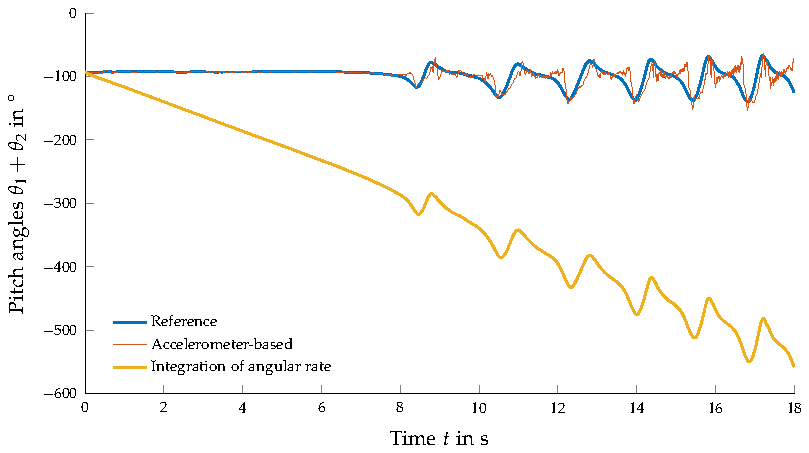
\includegraphics[width=\textwidth]{images/experiment_1.tikz}
	\caption{Pitch angle of the right shank - Comparison}
	\label{fig:experiment_1}
\end{figure}

%\begin{figure}
%	\centering
%	\setlength\figureheight{7cm} 
%	\setlength\figurewidth{\textwidth}
%	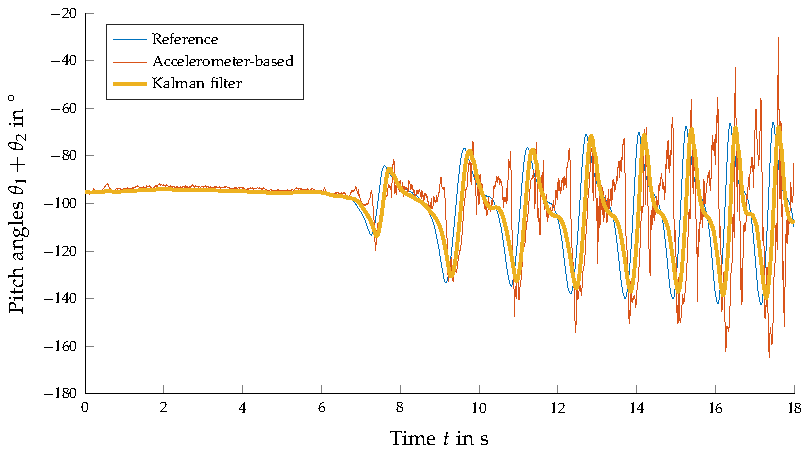
\includegraphics[width=\textwidth]{images/experiment_2.tikz}
%	\caption{Pitch angle of the right shank - Comparison}
%	\label{fig:experiment_2}
%\end{figure}
%
%\begin{figure}
%	\centering
%	\setlength\figureheight{7cm} 
%	\setlength\figurewidth{\textwidth}
%	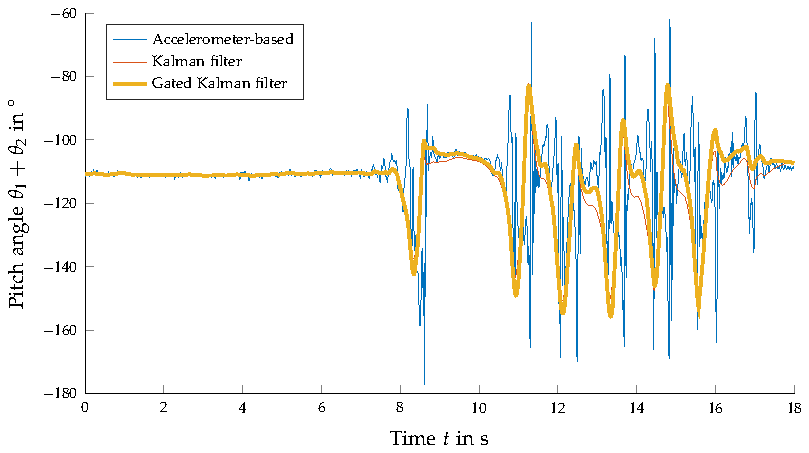
\includegraphics[width=\textwidth]{images/experiment_3.tikz}
%	\caption{Pitch angle of the right shank - Comparison}
%	\label{fig:experiment_4}
%\end{figure}

\section{Discussion}

